\subsection{Einleitung}
Das GUI vom Proximety ist so aufgebaut, dass nur die für den aktuellen Context unerlässlichen Informationen dargestellt werden. So wird sichergestellt, dass der Benutzer nicht durch Informationen verwirrt wird, welche er für die aktuelle Aktion nicht gebrauchen kann.

Durch das Betätigen des Zurück-Knopfes kommt man im Applikationsfluss zurück auf die letzte Maske. Sollte sich der Benutzer auf dem Main Screen befinden, löst ein Drücken des Zurück-Knopfes das Schliessen der Applikation aus. 

Eingaben des Benutzers werden immer auf die Gültigkeit überprüft und mit einer Hinweis-Meldung behandelt. Ein erfolgreiches vorwärts gerichtetes Verlassen der Screens ist erst möglich, wenn alle Eingaben gültig sind. Zusätzlich zur Meldung wird noch das Eingabe-Feld markiert, in welchem der Fehler aufgetreten ist.

Im nachfolgenden Flow Chart wird der Fluss der Applikation durch die einzelnen Masken visualisiert.

\begin{figure}[hp]
	\centering
		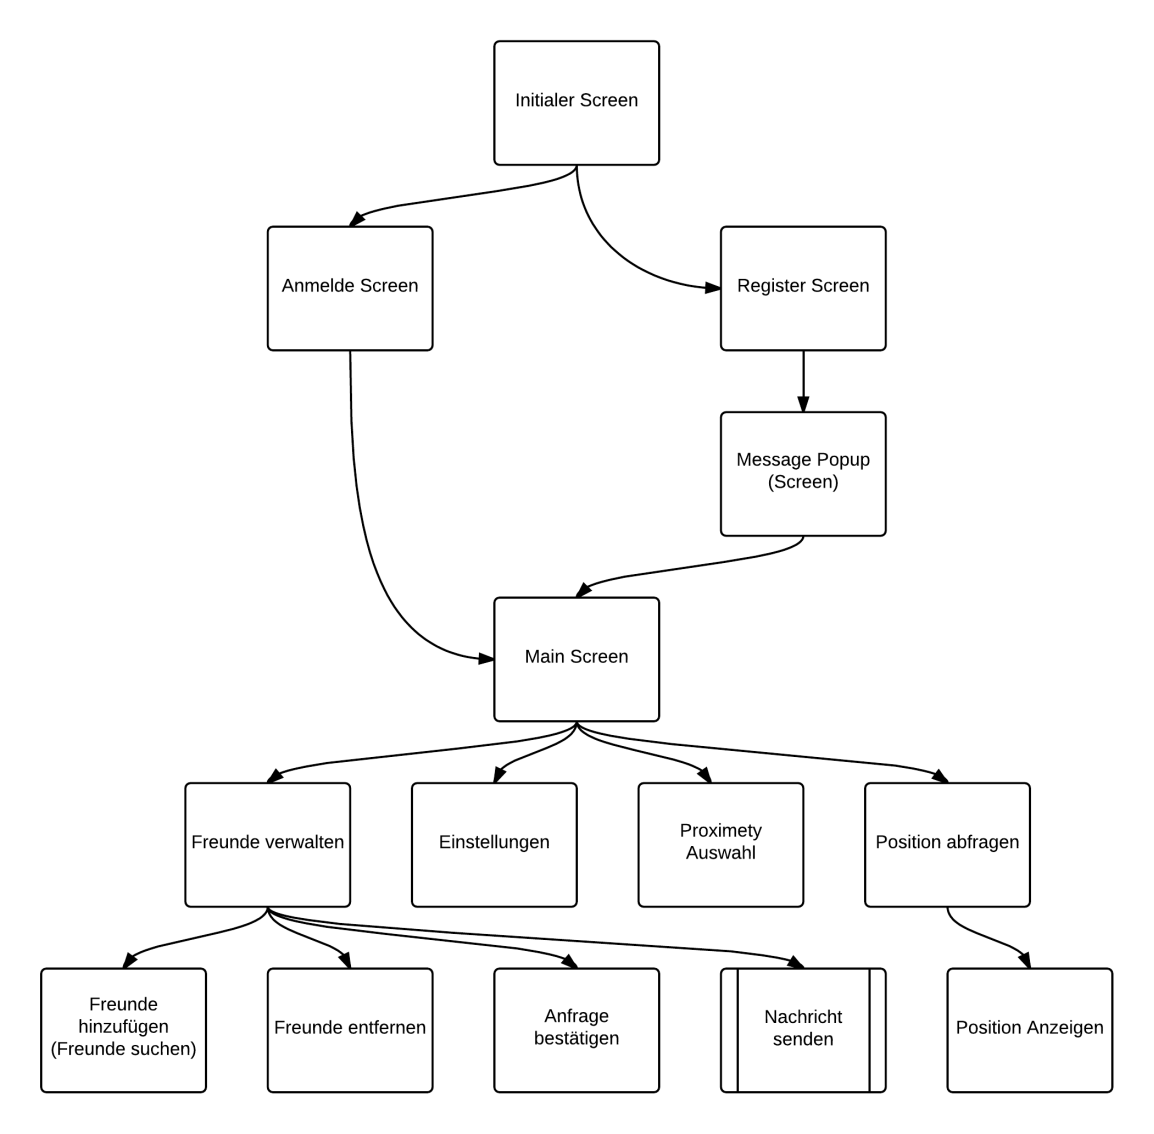
\includegraphics[scale=0.4]{ProximetyUIFlow.png}
	\caption{Design Flow Diagramm}
	\label{fig:ProximetyUIFlow}
\end{figure}
\FloatBarrier